% ======================================================================
% Effects of Interference and Task-Switching Demands on Completion Time
% in D-KEFS Color-Word Interference
% Amanda Ta - PSY 410: Advanced Research Methods (San Diego State Univ.)
%
% LaTeX edition of the author's course paper. The prose is unchanged
% from the original Word manuscript; only the typesetting is new.
% Figure 1 is drawn in-document with pgfplots from the reported
% descriptive statistics (n = 15; error bars are 95% confidence
% intervals), so no external figure files are needed.
%
% To compile: pdflatex Ta_PSY410_Experiment1.tex (run twice so the
% Table/Figure cross-references resolve). Requires the apa7 document
% class and pgfplots - both ship with standard TeX Live / MiKTeX
% installs (TeX Live: tlmgr install apa7 pgfplots).
% ======================================================================

\documentclass[stu,floatsintext]{apa7}

\usepackage[utf8]{inputenc}
\usepackage{booktabs}    % professional-looking tables
\usepackage{graphicx}    % included figures, if ever needed
\usepackage{pgfplots}    % Figure 1, drawn from the reported statistics
\pgfplotsset{compat=1.18}
\usepackage{hyperref}    % clickable URLs

\definecolor{barpink}{HTML}{F06292}
\definecolor{barpinkedge}{HTML}{AD1457}

\title{Effects of Interference and Task-Switching Demands on Completion Time in D-KEFS Color-Word Interference}
\shorttitle{Interference and Task-Switching in D-KEFS}
\author{Amanda Ta}
\affiliation{Department of Psychology, San Diego State University}
\course{PSY 410: Advanced Research Methods}
\professor{Claire Murphy}
\duedate{September 28, 2026}

\abstract{This study examined executive control by comparing performance across the four conditions of the Delis-Kaplan Executive Function System (D-KEFS) Color-Word Interference Test (CWIT): Color Naming, Word Reading, Inhibition, and Inhibition/Switching. Fifteen undergraduate students, each from San Diego State University completed all four conditions in the standard fixed order, and completion time in seconds was recorded for each. A one-way repeated-measures analysis of variance (ANOVA) revealed a significant effect of condition on completion time, $F(3, 42) = 46.98$, $p < .001$, partial $\eta^2 = .77$. Because Mauchly's test indicated a violation of sphericity, $\chi^2(5) = 22.66$, $p < .001$, degrees of freedom were corrected using the Greenhouse-Geisser estimate ($\varepsilon = .53$); the corrected effect remained significant, $p < .001$. Bonferroni-adjusted pairwise comparisons showed that completion time increased significantly across every pair of conditions except Inhibition versus Inhibition/Switching, which did not differ significantly. These findings are consistent with the expected pattern of increasing cognitive demand across the CWIT conditions, with the two inhibition-based conditions imposing comparably high executive load relative to the baseline naming and reading conditions.}

\begin{document}
\maketitle

\section{Methods}

\subsection{Participants}

Participants were 15 undergraduate students each enrolled in the PSY 410: Research Methods course at San Diego State University. No additional demographic information was collected.

\subsection{Materials}

Executive functioning was assessed using the Color-Word Interference Test (CWIT) from the Delis-Kaplan Executive Function System (D-KEFS; Delis et al., 2001). The CWIT consists of four conditions administered on a single stimulus page: Color Naming, in which participants name the colors of printed color patches; Word Reading, in which participants read color words printed in black ink; Inhibition, in which participants name the ink color of color words printed in an incongruent color (e.g., the word ``red'' printed in blue ink), requiring inhibition of the more automatic word-reading response; and Inhibition/Switching, in which participants alternate between naming the ink color and reading the word itself, depending on whether the item is boxed. Completion time in seconds served as the dependent variable for each condition, with slower times reflecting poorer performance.

\subsection{Procedure}

All participants completed the four CWIT conditions individually in the standard, fixed administration order: Color Naming, Word Reading, Inhibition, and Inhibition/Switching. An examiner timed each condition with a stopwatch and recorded the time to completion, in seconds, immediately after each trial. Because every participant completed all four conditions, the data were analyzed using a one-way repeated-measures design with condition (Color Naming, Word Reading, Inhibition, Inhibition/Switching) as the within-subjects factor and completion time as the dependent variable. All statistical analyses, including the repeated-measures analysis of variance, Mauchly's test of sphericity, the Greenhouse-Geisser correction, and Bonferroni-adjusted post hoc comparisons, were conducted in R (R Core Team, 2026).

\section{Results}

Descriptive statistics for completion time (in seconds) across the four CWIT conditions are presented in Table~\ref{tab:times} and Figure~\ref{fig:times}. Mean completion time increased monotonically from Word Reading to Color Naming to Inhibition to Inhibition/Switching, consistent with increasing executive demand across conditions.

\begin{table}[htbp]
  \centering
  \caption{Mean Completion Time (in Seconds) by CWIT Condition}
  \label{tab:times}
  \begin{tabular}{lcc}
    \toprule
    Condition & \textit{M} & \textit{SD} \\
    \midrule
    Word Reading         & 21.64 &  3.48 \\
    Color Naming         & 31.27 &  5.44 \\
    Inhibition           & 52.80 & 10.78 \\
    Inhibition/Switching & 59.12 & 17.06 \\
    \bottomrule
  \end{tabular}
\end{table}

A one-way repeated-measures ANOVA was conducted to compare completion time across the four CWIT conditions. The effect of condition was significant, $F(3, 42) = 46.98$, $p < .001$, partial $\eta^2 = .77$, indicating that completion time differed reliably across conditions. Mauchly's test indicated that the assumption of sphericity was violated, $W = .17$, $\chi^2(5) = 22.66$, $p < .001$, so degrees of freedom were corrected using the Greenhouse-Geisser estimate ($\varepsilon = .53$). The condition effect remained significant under this correction, $F(1.58, 22.07) = 46.98$, $p < .001$.

Bonferroni-adjusted pairwise comparisons were conducted to follow up the omnibus effect. Completion time was significantly faster for Word Reading than for Color Naming, $t(14) = -7.19$, $p < .001$; Inhibition, $t(14) = -12.95$, $p < .001$; and Inhibition/Switching, $t(14) = -8.36$, $p < .001$. Color Naming was also significantly faster than Inhibition, $t(14) = -8.63$, $p < .001$, and Inhibition/Switching, $t(14) = -6.09$, $p < .001$. Inhibition and Inhibition/Switching did not differ significantly from one another, $t(14) = -1.27$, $p = 1.00$. Taken together, these results indicate that the two inhibition-based conditions each required significantly more time to complete than the baseline naming and reading conditions, but did not differ significantly from each other.

\begin{figure}[htbp]
  \centering
  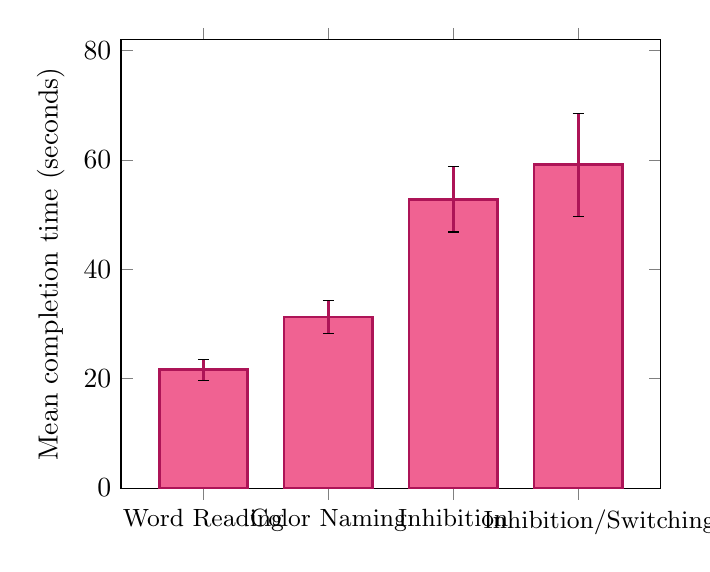
\begin{tikzpicture}
    \begin{axis}[
      ybar,
      bar width=32pt,
      ymin=0, ymax=82,
      ylabel={Mean completion time (seconds)},
      symbolic x coords={Word Reading, Color Naming, Inhibition, Inhibition/Switching},
      xtick=data,
      xticklabel style={font=\small, text width=2.4cm, align=center},
      enlarge x limits=0.22,
      error bars/y dir=both,
      error bars/y explicit,
      error bars/error bar style={line width=1pt},
    ]
      \addplot [fill=barpink, draw=barpinkedge, line width=1pt] coordinates {
        (Word Reading,         21.64) +- (1.93, 1.93)
        (Color Naming,         31.27) +- (3.01, 3.01)
        (Inhibition,           52.80) +- (5.97, 5.97)
        (Inhibition/Switching, 59.12) +- (9.45, 9.45)
      };
    \end{axis}
  \end{tikzpicture}
  \caption{Mean Completion Time by CWIT Condition}
  \figurenote{Error bars represent 95\% confidence intervals. $N = 15$.}
  \label{fig:times}
\end{figure}

\section{References}

\noindent\hangindent=0.5in Delis, D. C., Kaplan, E., \& Kramer, J. H. (2001). \textit{Delis-Kaplan Executive Function System (D-KEFS).} Pearson.

\noindent\hangindent=0.5in R Core Team. (2026). \textit{R: A language and environment for statistical computing} (Version 4.4) [Computer software]. R Foundation for Statistical Computing. \url{https://www.R-project.org/}

\end{document}
